\documentclass[a4paper,11pt]{article}
\pdfoutput=1 % if your are submitting a pdflatex (i.e. if you have
             % images in pdf, png or jpg format)

\usepackage{jheppub} % for details on the use of the package, please
                     % see the JHEP-author-manual
\usepackage{amsmath}
\usepackage[T1]{fontenc} % if needed
\usepackage{graphicx}
\usepackage{tikz}
\usetikzlibrary{automata, positioning}

\title{Financial Market Modeling using Hidden Markov Models}


%% %simple case: 2 authors, same institution
%% \author{A. Uthor}
%% \author{and A. Nother Author}
%% \affiliation{Institution,\\Address, Country}

% more complex case: 4 authors, 3 institutions, 2 footnotes
\author{Elliot Golias}
%\author[c]{S. Econd,}
%\author[a,2]{T. Hird\note{Also at Some University.}}
%\author[a,2]{and Fourth}

% The "\note" macro will give a warning: "Ignoring empty anchor..."
% you can safely ignore it.

%\affiliation[a]{One University,\\some-street, Country}
%\affiliation[b]{Another University,\\different-address, Country}
%\affiliation[c]{A School for Advanced Studies,\\some-location, Country}

% e-mail addresses: one for each author, in the same order as the authors
\emailAdd{elliot.golias@gmail.com}
%\emailAdd{second@asas.edu}
%\emailAdd{third@one.univ}
%\emailAdd{fourth@one.univ}




\abstract{This paper presents a comprehensive study on the application of Hidden Markov Models (HMMs) 
for sequential data analysis. The project involves training HMMs, evaluating their performance, and 
utilizing them for tasks such as sequence classification and prediction. By employing probabilistic 
modeling techniques, the project demonstrates the effectiveness of HMMs in capturing underlying 
patterns in sequential financial data. The results highlight the potential of HMMs for various real-world 
applications requiring sequential data analysis.}



\begin{document} 
\maketitle
\flushbottom

%%%%%%%%%%%%%%%%%%%%%%%%%%%%%%%%%%%%%%%%%%%%%%%
\section{Introduction}
%%%%%%%%%%%%%%%%%%%%%%%%%%%%%%%%%%%%%%%%%%%%%%%
\label{sec:intro}

Quantitative finance is a field that heavily relies on mathematical models and statistical techniques to
analyze financial markets and make informed investment decisions. In recent years, the application of
machine learning algorithms has gained significant attention in quantitative finance, enabling
practitioners to extract valuable insights and build predictive models from vast amounts of financial
data. One powerful and widely used machine learning framework in quantitative finance is the hidden
Markov model (HMM).

Hidden Markov models are probabilistic models that capture the dynamics of sequential
data by modeling the underlying hidden states and their observable outputs. They are particularly suitable for modeling time series data, where the observed data is influenced by unobserved or hidden factors that evolve over time. HMMs have found numerous applications in various domains, including speech recognition, natural language processing, bioinformatics, and, more recently, quantitative finance.

At its core, a hidden Markov model consists of two fundamental components: the hidden states and the observable outputs. The hidden states represent the underlying, unobserved factors that drive the system's dynamics, while the observable outputs represent the observed data points associated with each hidden state. The relationship between the hidden states and the observable outputs is governed by two key probability distributions: the state transition probabilities and the emission probabilities.

In the context of quantitative finance, hidden Markov models provide a flexible and powerful framework for modeling financial time series data. By capturing the latent market regimes or hidden patterns within the data, HMMs can offer valuable insights into the dynamics of financial markets, such as the identification of bull or bear market phases, regime shifts, or the presence of market anomalies.

Machine learning techniques, combined with hidden Markov models, can further enhance the modeling capabilities in quantitative finance. The estimation and inference procedures in HMMs can be enhanced using various machine learning algorithms, such as the expectation-maximization (EM) algorithm or the Baum-Welch algorithm, which enable the model to learn the parameters from the observed data and make probabilistic predictions.

In this research paper, we explore the application of hidden Markov models in quantitative finance and their integration with machine learning techniques. We investigate how HMMs can be used to model financial time series data, make predictions, and assist in investment decision-making. We also explore the challenges and opportunities associated with HMMs in quantitative finance, including model selection, parameter estimation, and model validation.

The remainder of this paper is organized as follows. Section 2 provides a detailed overview of hidden Markov models, including the mathematical formulation and key inference algorithms. Section 3 presents the application of HMMs in quantitative finance, discussing their use in modeling financial time series data and predictive analytics. Section 4 discusses the integration of machine learning techniques with HMMs, highlighting the potential improvements and challenges. Finally, Section 5 concludes the paper with a summary and future research directions.


%%%%%%%%%%%%%%%%%%%%%%%%%%%%%%%%%%%%%%%%%%%%%%%
\section{Data Collection}
%%%%%%%%%%%%%%%%%%%%%%%%%%%%%%%%%%%%%%%%%%%%%%%
\label{sec:data_collection}

%%%%%%%%%%%%%%%%%%%%%%%%%%%%%%%%%%%%%%%%%%%%%%%
\section{Hidden Markov Models}
%%%%%%%%%%%%%%%%%%%%%%%%%%%%%%%%%%%%%%%%%%%%%%%
\label{sec:HHMs}

%%%%%%%%%%%%%%%%%%%%%%%%%%%%%%%%%%%%%%%%%%%%%%%
\subsection{Introduction to Discrete-Time Markov Chains}
%%%%%%%%%%%%%%%%%%%%%%%%%%%%%%%%%%%%%%%%%%%%%%%
\label{sec:Intro-to-HHM}

A discrete-time Markov chain with a finite set of states is a stochastic model widely used in financial modeling to analyze systems with sequential dependencies. It is characterized by the following mathematical components:

1. \textbf{State Space}: Let $S = \{S_1, S_2, \ldots, S_n\}$ be the set of states in the Markov chain. Each state represents a distinct condition or regime of the financial system under consideration. In financial modeling, states could represent market regimes (e.g., bull, bear, or volatile markets), economic conditions (e.g., expansion or recession), or other relevant factors.

2. \textbf{State Transition Probability Matrix}: The state transition probability matrix, denoted by $P$, is an $n \times n$ matrix, where $P_{ij}$ represents the probability of transitioning from state $S_i$ to state $S_j$. The matrix $P$ satisfies the following properties:
\[
P_{ij} \geq 0 \quad \text{for all } i, j \quad \text{(non-negativity)}
\]
\[
\sum_{j=1}^{n} P_{ij} = 1 \quad \text{for all } i \quad \text{(row sum equals 1)}
\]
These properties ensure that the transition probabilities are valid probabilities and that the system moves from one state to another at each time step.

3. \textbf{Initial State Probability Vector}: The initial state probability vector, denoted by $\pi$, is a row vector of length $n$, where $\pi_i$ represents the probability of starting in state $S_i$. The vector $\pi$ satisfies the following properties:
\[
\pi_i \geq 0 \quad \text{for all } i \quad \text{(non-negativity)}
\]
\[
\sum_{i=1}^{n} \pi_i = 1 \quad \text{(sum equals 1)}
\]
These properties ensure that the initial probabilities represent a valid probability distribution over the states.

4. \textbf{Homogeneity}: A Markov chain is said to be *homogeneous* if the transition probabilities do not depend on time. In this case, the matrix $P$ remains constant over time. This assumption simplifies modeling and analysis, but it may not always hold in financial markets where transition probabilities can change over different time periods.

5. \textbf{State Probabilities}: The state probabilities at each time step can be computed using the recursive relationship:
\[
X_{k+1} = X_k \cdot P
\]
where $X_k$ is a row vector of length $n$ representing the probabilities of being in each state at time $k$. This relationship allows us to determine the probabilities of the system being in different states as time progresses.

6. \textbf{Stationary Distribution}: The long-term behavior of a Markov chain is characterized by its stationary distribution. A stationary distribution, denoted by $\pi^*$, is a row vector of length $n$ that satisfies the following properties:
\[
\pi^* \cdot P = \pi^* \quad \text{(probability conservation)}
\]
\[
\sum_{i=1}^{n} \pi^*_i = 1 \quad \text{(sum equals 1)}
\]
The stationary distribution provides the long-term probabilities of being in each state, regardless of the initial state. For a homogeneous Markov chain, the state probabilities converge to the stationary distribution as time progresses. In financial modeling, the stationary distribution can provide valuable insights into the long-term behavior of market regimes or economic conditions.

Discrete-time Markov chains serve as powerful tools for financial modeling and analysis. They allow us to study probabilistic transitions between different states, make predictions about future states, estimate risk and return characteristics, and guide decision-making processes. Markov chains provide a mathematical framework for capturing the sequential dependencies in financial data and analyzing their dynamics.

%%%%%%%%%%%%%%%%%%%%%%%%%%%%%%%%%%%%%%%%%%%%%%%
\subsection{Hidden Markov Models (HHMs)}
%%%%%%%%%%%%%%%%%%%%%%%%%%%%%%%%%%%%%%%%%%%%%%%
\label{sec:HHM}

Consider the hidden Markov model represented graphically in \ref{HMM-Graph}. This representation
contains three states ($S_1$, $S_2$, $S_3$) and three corresponding observations ($O_1$, $O_2$, $O_3$)
The transitions between the states are represented by arrows, and the transition probabilities
are given by $P_{ij}$.
\begin{figure}[h]
    \label{HMM-Graph}
    \centering
    
    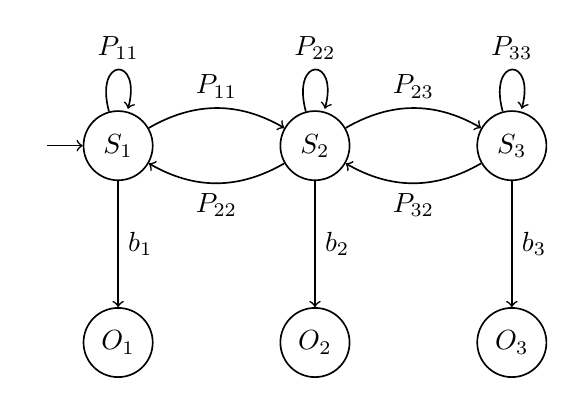
\begin{tikzpicture}[->, auto, node distance=2.5cm, semithick, initial text={}]
        % Hidden states
        \node[state, initial] (s1) {$S_1$};
        \node[state, right of=s1] (s2) {$S_2$};
        \node[state, right of=s2] (s3) {$S_3$};
    
        % Observations
        \node[state, below of=s1] (o1) {$O_1$};
        \node[state, below of=s2] (o2) {$O_2$};
        \node[state, below of=s3] (o3) {$O_3$};
    
        % Transitions
        \draw (s1) edge[bend left] node{$P_{11}$} (s2)
            (s2) edge[bend left] node{$P_{22}$} (s1)
            (s2) edge[bend left] node{$P_{23}$} (s3)
            (s3) edge[bend left] node{$P_{32}$} (s2)
            (s1) edge[loop above] node{$P_{11}$} (s1)
            (s2) edge[loop above] node{$P_{22}$} (s2)
            (s3) edge[loop above] node{$P_{33}$} (s3);
    
        % Emissions
        \draw (s1) edge node[right]{$b_{1}$} (o1)
            (s2) edge node[right]{$b_{2}$} (o2)
            (s3) edge node[right]{$b_{3}$} (o3);
    \end{tikzpicture}

    \caption{Illustration of an example of a hidden Markov model.}
\end{figure}

%%%%%%%%%%%%%%%%%%%%%%%%%%%%%%%%%%%%%%%%%%%%%%%
\subsection{The Baum-Welch Algorithm}
%%%%%%%%%%%%%%%%%%%%%%%%%%%%%%%%%%%%%%%%%%%%%%%
\label{sec:baum-welch}

The Baum-Welch algorithm, also known as the forward-backward algorithm or the expectation-maximization 
(EM) algorithm, is a popular method used to estimate the unknown parameters of a hidden Markov model (HMM). 
Specifically, it is employed to estimate the emission and transition probabilities of the HMM given only 
the observed data.

Let's consider a discrete-time hidden Markov model with a finite set of states and observations. The key 
components of the HMM are the state space $S$, the observation space $O$, the state transition probability 
matrix $A$, the observation emission probability matrix $B$, and the initial state probability vector 
$\pi$.

The Baum-Welch algorithm iteratively maximizes the likelihood of the observed data by adjusting the model 
parameters $A$, $B$, and $\pi$. The algorithm involves two main steps: the \textbf{expectation step (E-step)} 
and the \textbf{maximization step (M-step)}.

1. \textbf{Expectation Step (E-step)}: In this step, the algorithm calculates the expected number of times 
the HMM is in a particular state or transitions between states, given the observed data and the current parameter 
estimates. It uses the forward-backward procedure to compute the \textbf{forward probabilities} and 
\textbf{backward probabilities}.

   - The \textbf{forward probabilities}, denoted by $\alpha$, represent the probability of being in a particular 
   state at a given time, given the observed sequence up to that time. They are calculated using the forward 
   algorithm.

   - The \textbf{backward probabilities}, denoted by $\beta$, represent the probability of observing the 
   remaining sequence from a particular state at a given time. They are calculated using the backward 
   algorithm.

   Using these probabilities, the algorithm computes the \textbf{expected number of state transitions} and the 
   \textbf{expected number of emissions}, which are used in the subsequent maximization step.

2. \textbf{Maximization Step (M-step)}: In this step, the algorithm updates the model parameters based on the expected counts obtained from the E-step.

   - The \textbf{transition probabilities} $A$ are updated by normalizing the expected number of state transitions.

   - The \textbf{emission probabilities} $B$ are updated by normalizing the expected number of emissions.

   - The \textbf{initial state probabilities} $\pi$ are updated by setting them equal to the expected number of times the HMM starts in each state, normalized to sum to 1.

   These updates improve the parameter estimates and increase the likelihood of the observed data. The E-step and M-step are iterated until convergence, where the likelihood of the observed data reaches a maximum or the parameter estimates stabilize.

The Baum-Welch algorithm is an unsupervised learning algorithm, meaning it does not require labeled training data. It is widely used in applications such as speech recognition, bioinformatics, and finance, where HMMs are used to model sequential data with hidden states. The algorithm allows for the estimation of the underlying hidden structure based solely on the observed data.

The Baum-Welch algorithm provides a powerful tool for training hidden Markov models and estimating the emission and transition probabilities. By iteratively maximizing the likelihood of the observed data, it enables the HMM to capture the underlying dynamics of the system and make accurate predictions or generate new sequences of observations.

%%%%%%%%%%%%%%%%%%%%%%%%%%%%%%%%%%%%%%%%%%%%%%%
\subsection{The Viterbi Algorithm}
%%%%%%%%%%%%%%%%%%%%%%%%%%%%%%%%%%%%%%%%%%%%%%%
\label{sec:viterbi}

The Viterbi algorithm is a dynamic programming algorithm used to find the most likely sequence of hidden states in a hidden Markov model (HMM) given an observed sequence. It is particularly useful when dealing with problems involving hidden or unobservable states.

Let's consider a discrete-time hidden Markov model with a finite set of states and observations. The key components of the HMM are the state space $S$, the observation space $O$, the state transition probability matrix $A$, the observation emission probability matrix $B$, and the initial state probability vector $\pi$.

The Viterbi algorithm is based on the principle of dynamic programming and involves the following steps:

1. \textbf{Initialization}: In this step, we initialize the algorithm by calculating the initial values for the Viterbi variables. We set the initial Viterbi variable $V_{1}(i)$ to the product of the initial state probability $\pi(i)$ and the emission probability $B_{i}(O_1)$ for each state $i$.

2. \textbf{Recursion}: In this step, we calculate the Viterbi variables for each time step from $t = 2$ to $T$, where $T$ is the length of the observed sequence. For each state $j$ at time step $t$, we compute the maximum value of the product of the previous Viterbi variable $V_{t-1}(i)$, the state transition probability $A_{ij}$, and the emission probability $B_{j}(O_t)$. We also keep track of the previous state that maximizes the value.

3. \textbf{Termination}: In this step, we determine the final hidden state sequence by selecting the state with the highest Viterbi variable $V_{T}(i)$. This represents the most likely state at the last time step.

4. \textbf{Backtracking}: In this step, we backtrack through the hidden state sequence by following the path of the highest Viterbi variables at each time step. This gives us the most likely sequence of hidden states that generated the observed sequence.

The Viterbi algorithm provides an efficient way to find the optimal sequence of hidden states in an HMM. By considering all possible state transitions and emission probabilities, it guarantees the discovery of the state sequence with the highest probability given the observed data.

The Viterbi algorithm is widely used in various applications, such as speech recognition, natural language processing, bioinformatics, and finance. In finance, it can be applied to decode market regimes, predict asset price movements, or identify hidden patterns in financial time series data.

The Viterbi algorithm is based on the principle of optimality and dynamic programming, enabling it to efficiently find the most likely hidden state sequence in an HMM. By leveraging the information from previous time steps, it avoids the need for exhaustive search and significantly reduces computational complexity.


%%%%%%%%%%%%%%%%%%%%%%%%%%%%%%%%%%%%%%%%%%%%%%%
\subsection{The Forward Algorithm}
%%%%%%%%%%%%%%%%%%%%%%%%%%%%%%%%%%%%%%%%%%%%%%%
\label{sec:forward}

The Forward algorithm is a dynamic programming algorithm used to compute the probability of an observed sequence in a hidden Markov model (HMM). It allows us to efficiently calculate the likelihood of the observed data given the model parameters.

Let's consider a discrete-time hidden Markov model with a finite set of states and observations. The key components of the HMM are the state space $S$, the observation space $O$, the state transition probability matrix $A$, the observation emission probability matrix $B$, and the initial state probability vector $\pi$.

The Forward algorithm involves the following steps:

1. \textbf{Initialization}: In this step, we initialize the algorithm by calculating the initial values for the forward variables. We set the forward variable $\alpha_1(i)$ to the product of the initial state probability $\pi(i)$ and the emission probability $B_{i}(O_1)$ for each state $i$.

2. \textbf{Recursion}: In this step, we calculate the forward variables for each time step from $t = 2$ to $T$, where $T$ is the length of the observed sequence. For each state $j$ at time step $t$, we compute the sum of the product of the previous forward variable $\alpha_{t-1}(i)$, the state transition probability $A_{ij}$, and the emission probability $B_{j}(O_t)$. This represents the probability of being in state $j$ at time $t$ given the observed sequence up to time $t$.

3. \textbf{Termination}: In this step, we sum up the final forward variables at time $T$, denoted as $P(O|\lambda)$, where $\lambda$ represents the model parameters of the HMM. This represents the probability of observing the entire sequence $O$ given the HMM.

The Forward algorithm provides an efficient way to calculate the likelihood of an observed sequence in an HMM. By considering all possible paths and summing up the probabilities of reaching each state at each time step, it gives us the overall probability of observing the sequence.

The Forward algorithm is widely used in various applications, such as speech recognition, natural language processing, bioinformatics, and finance. In finance, it can be applied to evaluate the likelihood of observing a given financial time series given a specific HMM model, allowing for model comparison, anomaly detection, or forecasting.

The Forward algorithm is based on the principle of dynamic programming, which exploits the overlapping subproblems and optimal substructure properties to efficiently compute the desired probability. By avoiding redundant computations and storing intermediate results, it significantly reduces the computational complexity compared to naive enumeration of all possible paths.

%%%%%%%%%%%%%%%%%%%%%%%%%%%%%%%%%%%%%%%%%%%%%%%
\subsection{The Backward Algorithm}
%%%%%%%%%%%%%%%%%%%%%%%%%%%%%%%%%%%%%%%%%%%%%%%
\label{sec:backward}

The Backward algorithm is a dynamic programming algorithm used to compute the probability of an observed sequence in a hidden Markov model (HMM). It complements the Forward algorithm by calculating the probability of the remaining observations given a particular state at a specific time.

Let's consider a discrete-time hidden Markov model with a finite set of states and observations. The key components of the HMM are the state space $S$, the observation space $O$, the state transition probability matrix $A$, the observation emission probability matrix $B$, and the initial state probability vector $\pi$.

The Backward algorithm involves the following steps:

1. \textbf{Initialization}: In this step, we initialize the algorithm by setting the backward variable $\beta_T(i)$ to 1 for each state $i$ at the final time step $T$.

2. \textbf{Recursion}: In this step, we calculate the backward variables for each time step from $t = T-1$ to 1. For each state $i$ at time step $t$, we compute the sum of the product of the next backward variable $\beta_{t+1}(j)$, the state transition probability $A_{ij}$, and the emission probability $B_{j}(O_{t+1})$. This represents the probability of observing the remaining sequence from time $t+1$ to $T$ given the current state $i$ at time $t$.

3. \textbf{Termination}: In this step, we compute the probability of observing the entire sequence $O$ given the HMM by summing up the product of the initial state probability $\pi(i)$, the emission probability $B_{i}(O_1)$, and the backward variable $\beta_1(i)$ for each state $i$. This represents the probability of observing the entire sequence $O$.

The Backward algorithm provides an efficient way to compute the likelihood of an observed sequence in an HMM. By considering the remaining observations given a particular state at a specific time and summing up the probabilities, it allows us to evaluate the overall probability of the observed sequence.

The Backward algorithm is widely used in various applications, such as speech recognition, natural language processing, bioinformatics, and finance. In finance, it can be applied to evaluate the likelihood of observing a given financial time series given a specific HMM model, allowing for model comparison, anomaly detection, or forecasting.

The Backward algorithm is based on the principle of dynamic programming, which exploits the overlapping subproblems and optimal substructure properties to efficiently compute the desired probability. By avoiding redundant computations and storing intermediate results, it significantly reduces the computational complexity compared to naive enumeration of all possible paths.

%%%%%%%%%%%%%%%%%%%%%%%%%%%%%%%%%%%%%%%%%%%%%%%
\section{Conclusions}
%%%%%%%%%%%%%%%%%%%%%%%%%%%%%%%%%%%%%%%%%%%%%%%
\label{sec:conclusions}


%\appendix
%\section{Some title}
%Please always give a title also for appendices.





%\acknowledgments

%This is the most common positions for acknowledgments. A macro is
%available to maintain the same layout and spelling of the heading.

%\paragraph{Note added.} This is also a good position for notes added
%after the paper has been written.





% The bibliography will probably be heavily edited during typesetting.
% We'll parse it and, using the arxiv number or the journal data, will
% query inspire, trying to verify the data (this will probalby spot
% eventual typos) and retrive the document DOI and eventual errata.
% We however suggest to always provide author, title and journal data:
% in short all the informations that clearly identify a document.

%\begin{thebibliography}{99}

%\bibitem{a}
%Author, \emph{Title}, \emph{J. Abbrev.} {\bf vol} (year) pg.

%\bibitem{b}
%Author, \emph{Title},
%arxiv:1234.5678.

%\bibitem{c}
%Author, \emph{Title},
%Publisher (year).


% Please avoid comments such as "For a review'', "For some examples",
% "and references therein" or move them in the text. In general,
% please leave only references in the bibliography and move all
% accessory text in footnotes.

% Also, please have only one work for each \bibitem.


%\end{thebibliography}
\end{document}
